\begin{tikzpicture}[line width=0.8pt, every node/.style={font=\small}, x=4cm, y=2.4cm]
  \draw (0,0) rectangle (1,1);
  \draw (0.25,0) -- (0.5,1);
  \draw (0.5,0) -- (0.75,1);
  \foreach \x in {0.25,0.5,0.75} { \draw (\x,1) -- (\x,1.04); \draw (\x,0) -- (\x,-0.04); }
  \node at (0.13,0.5) {$f$};
  \node at (0.5,0.5) {$g$};
  \node at (0.82,0.5) {$h$};
  \node[rotate=67, font=\scriptsize] at (0.31,0.5) {$s=\frac{1+t}{4}$};
  \node[rotate=67, font=\scriptsize] at (0.56,0.5) {$s=\frac{2+t}{4}$};
  \node[below] at (0,-0.04) {$0$};
  \node[below] at (0.25,-0.04) {$\tfrac14$};
  \node[below] at (0.5,-0.04) {$\tfrac12$};
  \node[below] at (0.75,-0.04) {$\tfrac34$};
  \node[below] at (1,-0.04) {$1$};
  \node[right] at (1.02,1) {$f*(g*h)$};
  \node[right] at (1.02,0) {$(f*g)*h$};
\end{tikzpicture}
